\section{The Web as a Platform} \label{chapter2:web-as-a-platform}

\begin{wrapfigure}{r}{0.2\textwidth}
  \vspace{-27pt}
  \begin{center}
    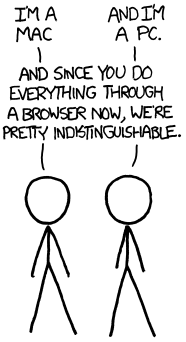
\includegraphics[width=0.18\textwidth]{../../ressources/Mac-PC.png}
  \end{center}
  \vspace{-20pt}
\end{wrapfigure}

Similarly to operating systems, Web browsers started as software products with extension capabilities with scripts and applications.
The distribution of an applications is limited only by the platform it can be deployed on.
The Web spreads the scalability of software distribution world wide with a near zero latency.
It eventually became the main distribution medium for software, and the wider market there can possibly be.
It led the Web to become the platform, replacing operating systems.

Now, with web services, or Software as a Service (SaaS), the distribution medium of software is so transparent that owning a software product to have an easier access is no longer relevant.
It stimulates a completely new business model based on a free access for the user, while claiming value for their data.
The next paragraphs present Javascript, the language that allowed this new business model to emerge.

\subsection{Javascript, The Language of the Web}

In the 80's with Moore's law predicting exponential increase in hardware performance, reducing development time became more profitable than reducing hardware costs.
Higher-level languages replaced lower-level languages, because the economical gain in development time compensated the worsen performances.
Most of the now popular programming languages were released at this time, Python(1991), Ruby(1993), Java(1994), PHP(1995) and Javascript(1995).

Java thrived in the software industry.
However, Java lose the hype that drove the community innovation and creativity, and now struggles to keep up with the latest trends in software development.
On the contrary, Ruby on Rails emerged from an industrial context, but is now open source, and backed by a strong community that makes it evolve and mature.
Other languages like Python and PHP, bloomed, grew within a strong community, and were later adopted by the industry for web development.
Django, the Python web frameworks, is used to develop many web applications in industrial contexts.
And Wordpress, a PHP publishing platform, is an economical success.
These examples show that the involvement of the community is critical for the adoption, evolution and maturation of a language.

Since a few years, Javascript is slowly becoming the main language for web development.
It is the only choice in the browser.
This position became an incentive to make it fast (V8, ASM.js) and convenient (ES6, ES7).
And since 2009, it is present on the server as well with Node.js
This omnipresence became an advantage.
It allows to develop and maintain the whole application with the same language.

\subsubsection{Historical Context}

\cit{There are only two kinds of languages: the ones people complain about and the ones nobody uses}{B. Stroustrup\ftnt{http://www.stroustrup.com/bs_faq.html\#really-say-that}}

Javascript was created by Brendan Eich at Netscape around May 1995, and released to the public in September.
At the time, Java was quickly adopted as the default language for web servers development, and everybody was betting on pushing Java to the client as well.
The history proved them wrong.

Javascript was released as a scripting engine on Netscape Navigator and later on its concurrent, Internet Explorer.
The competition between the two was fragmenting the Web.
Web pages had to be designed for a specific browser.
To stop this fragmentation, Netscape submitted Javascript to Ecma International for standardization in November 1996.
ECMA International released ECMA-262 in June 1997, the first standard for Javascript - or ECMAScript.
A standard to which all browser should refer for their implementations.

The initial release of Javascript was designed in a rush, within 10 days, and targeted unexperienced developers.
For these reasons, the language was considered poorly designed and unattractive by the developer community.

\illustration{the ugly duckling}

{\fontfamily{phv}\fontseries{l}
\fontsize{10pt}{10pt}\selectfont
Why does Javascript suck?\ftnt{http://whydoesitsuck.com/why-does-javascript-suck/}
Is Javascript here to stay?\ftnt{http://www.javaworld.com/article/2077224/learn-java/is-javascript-here-to-stay-.html}
Why Javascript Is Doomed.\ftnt{http://simpleprogrammer.com/2013/05/06/why-javascript-is-doomed/}
Why JavaScript Makes Bad Developers.\ftnt{https://thorprojects.com/blog/Lists/Posts/Post.aspx?ID=1646}
JavaScript: The World's Most Misunderstood Programming Language\ftnt{http://www.crockford.com/javascript/javascript.html}
Why Javascript Still Sucks\ftnt{http://www.boronine.com/2012/12/14/Why-JavaScript-Still-Sucks/}
10 things we hate about JavaScript\ftnt{http://www.infoworld.com/article/2606605/javascript/146732-10-things-we-hate-about-JavaScript.html}
Why do so many people seem to hate Javascript?\ftnt{https://www.quora.com/Why-do-so-many-people-seem-to-hate-JavaScript}
}

But things evolved drastically since.
All web browsers include a Javascript interpreter, making Javascript the most ubiquitous runtime \cite{Flanagan2006}.
Any Javascript code is open, allowing the community to pick, improve and reproduce the best techniques \ftnt{http://blog.codinghorror.com/the-power-of-view-source/}.
Javascript is distributed freely, with all the tools needed to reproduce and experiment on the largest communication network in history.
All these reasons made the popularity of the Web and Javascript.

% \paragraph{Rising of the unpopular language}

\paragraph{}

\cit{When JavaScript was first introduced, I dismissed it as being not worth my attention. Much later, I took another look at it and discovered that hidden in the browser was an excellent programming language.}{Douglas Crockford}

Javascript was initially limited to short interactions on web pages.
The typical usage was to pre-validate forms on the client to avoid wasting wrongly formated requests to the server.
This situation hugely improved since the beginning of the language.
Nowadays, there is a lot of web-based application replacing desktop applications, like mail client, word processor, music player, graphics editor…

ECMA International released several version in the few years following the creation of Javascript.
The third version contributed to give Javascript a more complete and solid base as a programming language.
From this point on, the consideration for Javascript kept improving.

In 2005, James Jesse Garrett released \textit{Ajax: A New Approach to Web Applications}, a white paper coining the term Ajax \cite{Garrett2005}.
It uses Javascript to dynamically  reload the content inside a web page, hence improving the user experience.
It allows Javascript to develop richer applications inside the browser, from user interactions to network communications.
The first web applications to use Ajax were Gmail, and Google maps\footnote{A more in-depth analysis of the history of Ajax, given by late Aaron Swartz \url{http://www.aaronsw.com/weblog/ajaxhistory}}.
The community released Javascript framework to assist the development of these larger applications.
Prototype\ftnt{http://prototypejs.org/} and DOJO\ftnt{https://dojotoolkit.org/} are early famous examples, and later jQuery\ftnt{https://jquery.com/} and underscore\ftnt{http://underscorejs.org/}.

\illustration{Javascript with superpowers}

In 2004, the Web Hypertext Application Technology Working Group\ftnt{https://whatwg.org/} was formed to work on the fifth version of the HTML standard.
The name is misleading, it is really about giving Javascript superpowers like geolocation, storage, audio, video, and many mores.
The releases of HTML5 and ECMAScript 5, in 2008 and 2009, represent a mile-stone in the development of web-based applications.
Around the same time, Google released the Javascript interpreter V8 for its browser Chrome, improving drastically the execution performance.
Javascript became the \textit{defacto} programming language to develop on this rising application platform that is the Web.

\begin{figure}

\newcommand{\event}[3][10pt]{\chronoevent[markdepth=-#1]{#2}{#3}}
\setupchronoevent{textstyle=\scriptsize,datestyle=\tiny\bf,datesseparation=/,conversionmonth=false}
% \usr\share\texmf-dist\tex\generic\chronosys\chronosyschr.tex:533 +>
% \vspace{-6pt} % I added this line because the space between date and text is too large for scriptsize font.

\startchronology[align=left, startyear=1994,stopyear=2016, height=0pt, startdate=false, stopdate=false, arrow=false, box=true]
%
\chronograduation[event][dateselevation=10pt]{2}


\event[35pt]  {06/2015}     {ECMAScript v6.0}
\event[10pt]  {14/01/2015}  {io.js}
\event[110pt] {06/2011}     {ECMAScript V5.1}
\event[85pt]  {12/2009}     {ECMAScript v5.0}
\event[60pt]  {27/06/2009}  {Node.js}
\event[35pt]  {02/09/2008}  {V8}
\event[10pt]  {22/01/2008}  {HTML5 public draft}
\event[10pt]  {04/06/2004}  {WHATWG}
\event[110pt] {12/1999}     {ECMAScript v3.0}
\event[85pt]  {06/1998}     {ECMAScript v2.0}
\event[60pt]  {06/1997}     {ECMAScript v1.0}
\event[35pt]  {11/1996}     {ECMA Standardization}
\event        {05/1995}     {Javascript Creation}



\stopchronology
\end{figure}

\subsubsection{Current Situation}

The rise of Javascript is indisputable on the web, and seems to be rising in the software industry as well.
But it is difficult to give an accurate representation of the situation because the software industry often maintains a fog of war to try to keep an edge.
The following paragraphs report some efforts to clear up the situation.
% More detailed informations are available section \ref{appendix:langpop}.

\paragraph{Available Resources}

According to the TIOBE Programming Community index, Javascript ranks 8th, as of October 2015, and was the most rising language in 2014.
This index measure the popularity of a programming language with the number of results on many search engines.
However, this measure is controversial as the number of pages doesn't represent the number of readers.
Alternatively, Javascript ranks 7th on the PYPL, as of October 2015.
The PYPL index is based on Google trends to measure the number of requests on a programming language.
However, it is limited to Google searches.
From these indexes, the major programming languages are Java, then C/C++, C\# and Python.
Javascript seems not as popular as previously described.
The following paragraphs rectify this vision.

\nt{TODO graphical ranking of TIOBE and PYPL}

\paragraph{Developers Collaboration Platforms}

Online collaboration tools gives an indicator of the number of developers and project using certain languages.
Javascript is the most used language on \textit{Github}, the most important collaborative development platform, with around 9 millions users.
It represents more than 320 000 repositories, while the second language is Java with more than 220 000 repositories.
Javascript is the most cited language on \textit{StackOverflow}, the most important Q\&A platform for developers.
It represent more than 960 000 questions, while the second is Java with around 940 000 questions.
Additionnaly, Javascript has the most important and impressive package repository growth.
Moreover, Javascript is currently the second language used in open source projects, according to \textit{Black Duck Software}\ftnt{https://www.blackducksoftware.com/}.
C is first, C++ third and Java fourth.\ftnt{https://www.blackducksoftware.com/resources/data}
These four languages represent about 80\% of all programming language usage in open source communities.

\nt{TODO redo this graph, it is ugly.}
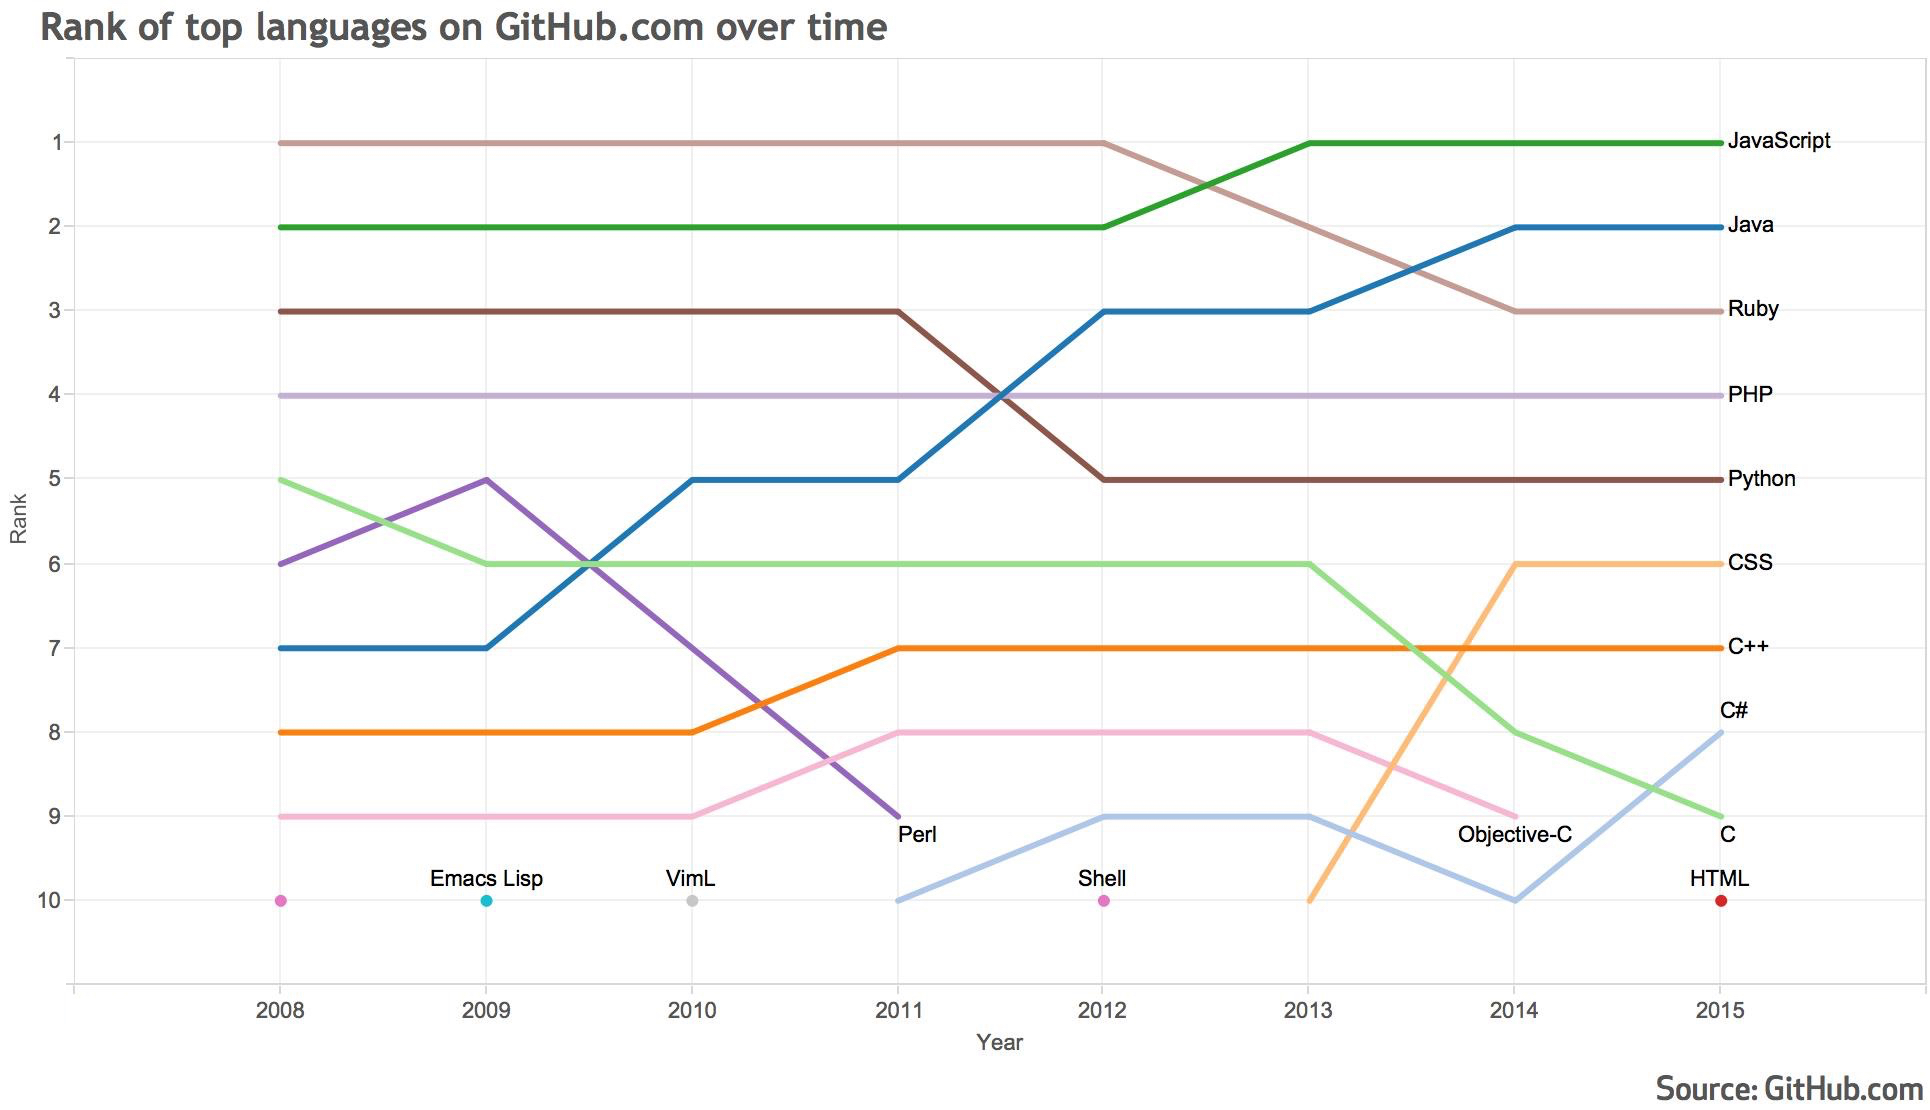
\includegraphics[width=0.9\linewidth]{../../../data/js-trends/github-ranks}\ftnt{https://github.com/blog/2047-language-trends-on-github}

\nt{TODO graphical ranking of the tags in StackOverflow}

\nt{TODO redo this graph, it is ugly.}
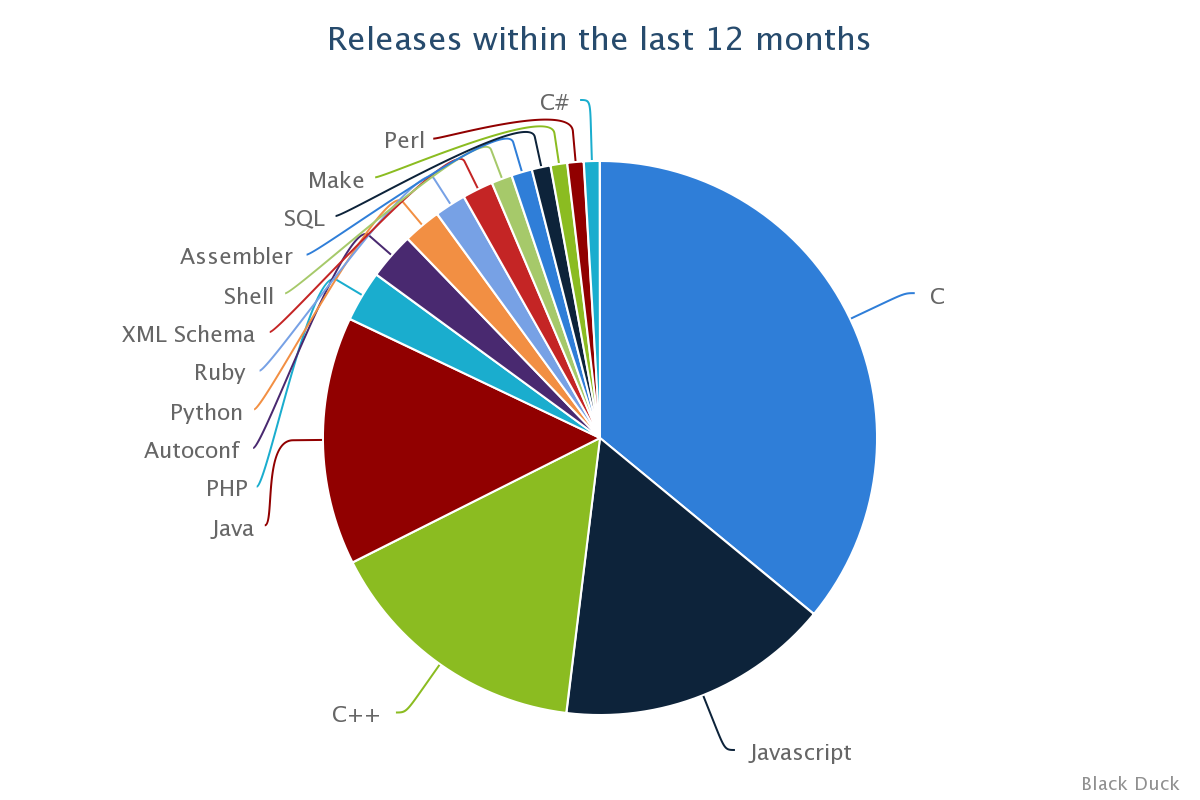
\includegraphics[width=0.9\linewidth]{../../../data/js-trends/black-duck-15}

\nt{TODO redo this graph, it is ugly.}
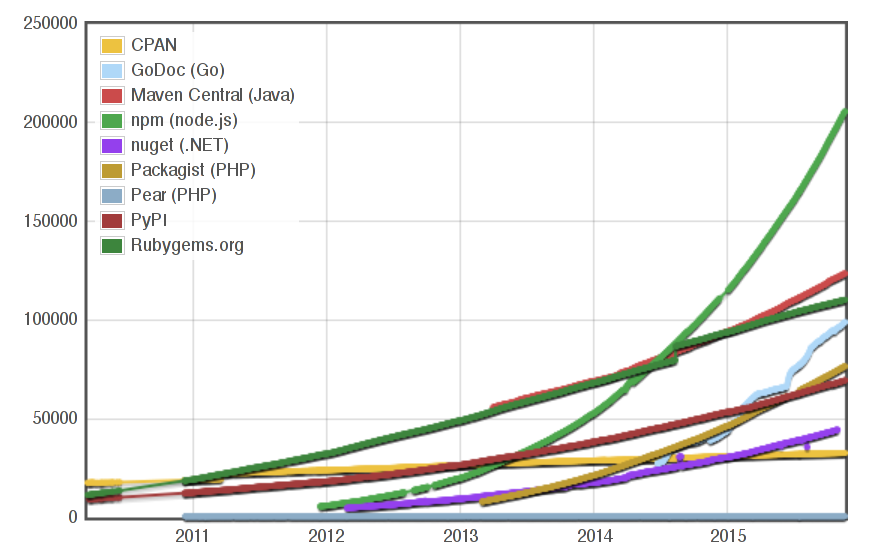
\includegraphics[width=0.9\linewidth]{../../../data/js-trends/modulecounts}

% \begin{figure}[h!]
% \begin{tikzpicture}
% [
%     pie chart,
%     slice type={c}{gray1},
%     slice type={js}{red},
%     slice type={cpp}{gray2},
%     slice type={java}{gray3},
%     slice type={php}{gray4},
%     slice type={autoconf}{gray5},
%     slice type={python}{gray6},
%     slice type={ruby}{gray1},
%     slice type={xml}{gray2},
%     slice type={sh}{gray3},
%     slice type={asm}{gray4},
%     slice type={sql}{gray5},
%     slice type={make}{gray6},
%     slice type={perl}{gray1},
%     slice type={csharp}{gray2},
%     pie values/.style={font={\small}},
%     scale=2
% ]

% \pie{}{%
%   34.80/c,%
%   15.45/js,%
%   15.13/cpp,%
%   14.02/java,%
%   2.87/php,%
%   2.65/autoconf,%
%   2.15/python,%
%   1.77/ruby,%
%   1.73/xml,%
%   1.18/sh,%
%   1.16/asm,%
%   1.07/sql,%
%   0.94/make,%
%   0.92/perl,%
%   0.90/csharp,%
% }

% \legend[shift={(1.3cm,0.9cm)}]{%
%   {C}/c,%
%   {Javascript}/js,%
%   {C++}/cpp,%
%   {Java}/java,%
%   {PHP}/php,%
%   {Autoconf}/autoconf,%
%   {Python}/python,%
%   {Ruby}/ruby,%
%   {XML Schema}/xml,%
%   {Shell}/sh,%
%   {Assembler}/asm,%
%   {SQL}/sql,%
%   {Make}/make,%
%   {Perl}/perl,%
%   {C\#}/csharp,%
% }
% \end{tikzpicture}
% \caption{Compilation results distribution}
% \end{figure}

\paragraph{Jobs}

The actors of the software industry tends to hide their activities trying to keep an edge on the competition.
The previous metrics represent the visible activity but are barely representative of the software industry.
The trends on job opportunities give some additional hints on the situation.
Javascript is the third most wanted skill, according to \textit{Indeed}\ftnt{http://www.indeed.com}, right after SQL and Java.\ftnt{http://www.indeed.com/jobtrends?q=Javascript\%2C+SQL\%2C+Java\%2C+C\%2B\%2B\%2C+C\%2FC\%2B\%2B\%2C+C\%23\%2C+Python\%2C+PHP\%2C+Ruby\&l=}
Moreover, according to \textit{breaz.io}\ftnt{https://breaz.io/}, Javascript developers get more opportunities than any other developers.
Javascript is increasingly adopted in the software industry.

\nt{TODO redo this graph, it is ugly.}
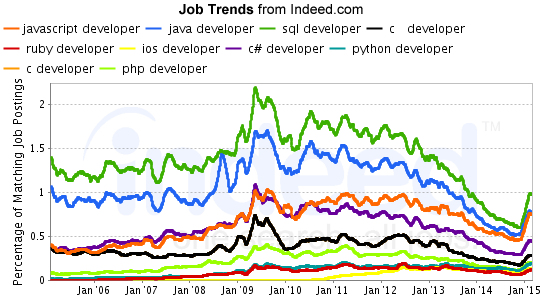
\includegraphics[width=0.9\linewidth]{../../../data/js-trends/jobgraph}

\paragraph{}

All these metrics represent different faces of the current situation of the Javascript adoption in the development community and industry.
It is widely used on the web, in open source projects, and in the software industry.
With the evolution of web applications development and increased interest in this domain, Javascript is assuredly one of most important language in the times to come.

This section presented the languages used to build web applications.
The next paragraphs presents the event-loop model used to develop Javascript web applications, both client and server-side.

\subsubsection{Event-Loop Execution Model} \ref{chapter2:web-as-a-platform:javascript:event-loop}

Javascript is often associated with an event-based paradigm to react to concurrent user interactions.
In 2009, Joyent released Node.js to build real-time web services with this paradigm.
It is a server-side implementation of Javascript based on an event-loop.
This event-based paradigm proved to be very efficient as well for a web service to react to concurrent requests.
This section presents the event-loop execution model, and the advantages of Javascript for this paradigm.

The event-loop efficiency comes from non-blocking communications, asynchronous execution, and cooperative scheduling.
It relies on a queue storing the messages received asynchronously.
The loop executes previously defined tasks to process these messages one after the other.
Each task can initiate new communications, leading in turn to the queuing of more messages, which trigger more tasks, and so on.
Each task is executed atomically and exclusively, until it yields execution, to continue with the next task in queue.

\nt{TODO schema of an event-loop}

\paragraph{Callbacks}

In Javascript, the asynchronous communications are initiated by function calls.
This asynchronous callee immediately returns to avoid waiting the result.
The task to process the result of the communication, and to continue the execution is a function passed as an argument to the callee.
This function is name a callback or a continuation.
A callback is a function passed as an argument to a callee, for the callee to transfer the control back to the caller after its execution, without the need for synchronization.

In this execution model, the execution is interrupted by asynchronous function calls.
It organizes the execution of callbacks causally, one after the other.
The input stream of data flows through a sequence of callbacks until the application outputs it.
The asynchronous execution flow is controlled by callbacks, and is organized similarly to a pipeline.
In this model, callbacks are the atoms of asynchronous execution flow control.
The next paragraph presents a more elaborate form of control.

\paragraph{Promises}

Since the asynchronous execution flow became more complicated on larger web application, many projects proposed improved asynchronous execution controls on top of callbacks.
The ECMAScript specification proposes Promises for such purpose.
It arranges sequence of causally related callbacks into neatly organized pipeline of callbacks communicating their result to the next.

Callbacks are said to be first class citizen.
They imply higher-order programming, which is part of functional programming.
Javascript features higher-order functions.

\paragraph{Closures}

For a callback to continue the execution without needing synchronization with the callee, it needs to have access to the initial context of the caller.
This context is linked with the function when passed to the callee.
The association of a function and its initial context is called a closure.

Higher-order programming is convenient for developers, as they allow great modularity in the implementation through \textit{e.g.} inversion of control.
It is presented in further details in section \ref{chapter3:software-maintainability}.
However, because the contexts are passed, and shared all over the implementation, this programming model needs a global memory for coordination.
As presented in the next section, this need is problematic to increase the concurrency of the execution.

This section presented Javascript as the language of the web, and its programming model.
The next section presents the realities and technical challenges to assure the performance of web services against billions of users.

\subsection{Highly Concurrent Web Servers}

The previous section presented Javascript, the prolific language to build the Web.
With SaaS, a Web service can scale world wide with near zero latency, and accessing it is as simple as distributing it world wide.
With this broad range of distribution, a new business model emerged, allowing free access for the user.
The usage exploded, and the software industry needed innovative solutions to cope with large network traffic.

\subsubsection{Scalable Concurrency}

The Internet allows communication at an unprecedented scale.
There is more than 16 billions connected devices, and it is growing fast\ftnt{http://blogs.cisco.com/news/cisco-connections-counter} \cite{Hilbert2011}.
A large web application like google search receives about 40 000 requests per seconds\ftnt{http://www.internetlivestats.com/google-search-statistics/}.
Such a Web application needs to be highly concurrent to manage this amount of simultaneous requests.
In the 2000s, the limit to break was 10 thousands simultaneous connections with a single commodity machine\ftnt{http://www.kegel.com/c10k.html}.
In the 2010s, the limit is set at 10 millions simultaneous connections\ftnt{http://c10m.robertgraham.com/p/manifesto.html}.
With the growing number of connected devices on the internet, concurrency is a very important property in the design of web applications.
Moreover, the concurrency needs to be scalable to adapt to this growth of audience, as explained in the next paragraph.

\paragraph{Scalability}

The traffic of a popular web application such as Google search remains stable because of its popularity.
The importance of the average traffic soften the occasional spikes.
However, the traffic of a less popular web application is much more uncertain.
For example, it might become viral when it is efficiently relayed in the media.
The load of the web application increases with the growth of audience.
The available resources needs to increase to meet this load.
This growth can be steady enough to plan the increase of resources ahead of time, or it might be erratic and challenging.
An application is scalable, if it is able to spread over resources proportionally as a reaction to the increasing growth of audience.

\subsubsection{Time-slicing and Parallelism}

Concurrency is achieved differently on hardware with a single or several processing units.
On a single processing unit, the tasks are executed sequentially, interleaved in time.
While on several processing units, the tasks are executed simultaneously, in parallel.
Parallel executions uses more processing units to reduce computing time over sequential execution.

If the tasks are independent, they can be executed in parallel as well as sequentially.
This parallelism is scalable, as the independent tasks can stretch the computation on the resources so as to meet the required performance.

However, the tasks within an application need to coordinate together to modify the application state.
This coordination limits the parallelism and imposes to execute some tasks sequentially.
It limits the scalability.
The type of possible concurrency, sequential or parallel, is defined by the interdependencies of the tasks.

The previous section presented the event-loop execution model used by Javascript.
As explained in the previous section, Javascript requires a global memory to coordinate the execution of the callbacks.
The event-loop is constrained within time-slicing concurrency to assure this coordination.

This thesis argues that the parallel equivalent to the event-loop is the pipeline execution model.
The next section presents this parallel execution model.

\subsubsection{Pipeline Execution Model}

The pipeline software architecture is composed of isolated stages communicating by message passing to leverage the parallelism of a multi-core hardware architectures.
It is well suited for streaming application, as the stream of data flows from stage to stage.
Each stage has an independent memory to hold its own state.
As the stages are independent, the state coordination between the stages are communicated along with the stream of data.

\nt{TODO schema of a pipeline}

Each stage is organized in a similar fashion than the event-loop presented in section \ref{chapter2:web-as-a-platform:javascript:event-loop}.
It receives and queues messages from upstream stages, processes them one after the other, and outputs the result to downstream stages.
The difference is that in the pipeline architecture, each task is executed on an isolated stage, whereas in the event-loop execution model, all tasks share the same queue, loop and memory store.

\paragraph{}

This section presented two execution models to build web services, the event-loop and the pipeline.
It presented briefly their similitudes and differences.
The next section details further the incompatibility in their model and the resulting economical consequences.
